
% Default to the notebook output style

    


% Inherit from the specified cell style.




    
\documentclass[11pt]{article}

    
    
    \usepackage[T1]{fontenc}
    % Nicer default font (+ math font) than Computer Modern for most use cases
    \usepackage{mathpazo}

    % Basic figure setup, for now with no caption control since it's done
    % automatically by Pandoc (which extracts ![](path) syntax from Markdown).
    \usepackage{graphicx}
    % We will generate all images so they have a width \maxwidth. This means
    % that they will get their normal width if they fit onto the page, but
    % are scaled down if they would overflow the margins.
    \makeatletter
    \def\maxwidth{\ifdim\Gin@nat@width>\linewidth\linewidth
    \else\Gin@nat@width\fi}
    \makeatother
    \let\Oldincludegraphics\includegraphics
    % Set max figure width to be 80% of text width, for now hardcoded.
    \renewcommand{\includegraphics}[1]{\Oldincludegraphics[width=.8\maxwidth]{#1}}
    % Ensure that by default, figures have no caption (until we provide a
    % proper Figure object with a Caption API and a way to capture that
    % in the conversion process - todo).
    \usepackage{caption}
    \DeclareCaptionLabelFormat{nolabel}{}
    \captionsetup{labelformat=nolabel}

    \usepackage{adjustbox} % Used to constrain images to a maximum size 
    \usepackage{xcolor} % Allow colors to be defined
    \usepackage{enumerate} % Needed for markdown enumerations to work
    \usepackage{geometry} % Used to adjust the document margins
    \usepackage{amsmath} % Equations
    \usepackage{amssymb} % Equations
    \usepackage{textcomp} % defines textquotesingle
    % Hack from http://tex.stackexchange.com/a/47451/13684:
    \AtBeginDocument{%
        \def\PYZsq{\textquotesingle}% Upright quotes in Pygmentized code
    }
    \usepackage{upquote} % Upright quotes for verbatim code
    \usepackage{eurosym} % defines \euro
    \usepackage[mathletters]{ucs} % Extended unicode (utf-8) support
    \usepackage[utf8x]{inputenc} % Allow utf-8 characters in the tex document
    \usepackage{fancyvrb} % verbatim replacement that allows latex
    \usepackage{grffile} % extends the file name processing of package graphics 
                         % to support a larger range 
    % The hyperref package gives us a pdf with properly built
    % internal navigation ('pdf bookmarks' for the table of contents,
    % internal cross-reference links, web links for URLs, etc.)
    \usepackage{hyperref}
    \usepackage{longtable} % longtable support required by pandoc >1.10
    \usepackage{booktabs}  % table support for pandoc > 1.12.2
    \usepackage[inline]{enumitem} % IRkernel/repr support (it uses the enumerate* environment)
    \usepackage[normalem]{ulem} % ulem is needed to support strikethroughs (\sout)
                                % normalem makes italics be italics, not underlines
    

    
    
    % Colors for the hyperref package
    \definecolor{urlcolor}{rgb}{0,.145,.698}
    \definecolor{linkcolor}{rgb}{.71,0.21,0.01}
    \definecolor{citecolor}{rgb}{.12,.54,.11}

    % ANSI colors
    \definecolor{ansi-black}{HTML}{3E424D}
    \definecolor{ansi-black-intense}{HTML}{282C36}
    \definecolor{ansi-red}{HTML}{E75C58}
    \definecolor{ansi-red-intense}{HTML}{B22B31}
    \definecolor{ansi-green}{HTML}{00A250}
    \definecolor{ansi-green-intense}{HTML}{007427}
    \definecolor{ansi-yellow}{HTML}{DDB62B}
    \definecolor{ansi-yellow-intense}{HTML}{B27D12}
    \definecolor{ansi-blue}{HTML}{208FFB}
    \definecolor{ansi-blue-intense}{HTML}{0065CA}
    \definecolor{ansi-magenta}{HTML}{D160C4}
    \definecolor{ansi-magenta-intense}{HTML}{A03196}
    \definecolor{ansi-cyan}{HTML}{60C6C8}
    \definecolor{ansi-cyan-intense}{HTML}{258F8F}
    \definecolor{ansi-white}{HTML}{C5C1B4}
    \definecolor{ansi-white-intense}{HTML}{A1A6B2}

    % commands and environments needed by pandoc snippets
    % extracted from the output of `pandoc -s`
    \providecommand{\tightlist}{%
      \setlength{\itemsep}{0pt}\setlength{\parskip}{0pt}}
    \DefineVerbatimEnvironment{Highlighting}{Verbatim}{commandchars=\\\{\}}
    % Add ',fontsize=\small' for more characters per line
    \newenvironment{Shaded}{}{}
    \newcommand{\KeywordTok}[1]{\textcolor[rgb]{0.00,0.44,0.13}{\textbf{{#1}}}}
    \newcommand{\DataTypeTok}[1]{\textcolor[rgb]{0.56,0.13,0.00}{{#1}}}
    \newcommand{\DecValTok}[1]{\textcolor[rgb]{0.25,0.63,0.44}{{#1}}}
    \newcommand{\BaseNTok}[1]{\textcolor[rgb]{0.25,0.63,0.44}{{#1}}}
    \newcommand{\FloatTok}[1]{\textcolor[rgb]{0.25,0.63,0.44}{{#1}}}
    \newcommand{\CharTok}[1]{\textcolor[rgb]{0.25,0.44,0.63}{{#1}}}
    \newcommand{\StringTok}[1]{\textcolor[rgb]{0.25,0.44,0.63}{{#1}}}
    \newcommand{\CommentTok}[1]{\textcolor[rgb]{0.38,0.63,0.69}{\textit{{#1}}}}
    \newcommand{\OtherTok}[1]{\textcolor[rgb]{0.00,0.44,0.13}{{#1}}}
    \newcommand{\AlertTok}[1]{\textcolor[rgb]{1.00,0.00,0.00}{\textbf{{#1}}}}
    \newcommand{\FunctionTok}[1]{\textcolor[rgb]{0.02,0.16,0.49}{{#1}}}
    \newcommand{\RegionMarkerTok}[1]{{#1}}
    \newcommand{\ErrorTok}[1]{\textcolor[rgb]{1.00,0.00,0.00}{\textbf{{#1}}}}
    \newcommand{\NormalTok}[1]{{#1}}
    
    % Additional commands for more recent versions of Pandoc
    \newcommand{\ConstantTok}[1]{\textcolor[rgb]{0.53,0.00,0.00}{{#1}}}
    \newcommand{\SpecialCharTok}[1]{\textcolor[rgb]{0.25,0.44,0.63}{{#1}}}
    \newcommand{\VerbatimStringTok}[1]{\textcolor[rgb]{0.25,0.44,0.63}{{#1}}}
    \newcommand{\SpecialStringTok}[1]{\textcolor[rgb]{0.73,0.40,0.53}{{#1}}}
    \newcommand{\ImportTok}[1]{{#1}}
    \newcommand{\DocumentationTok}[1]{\textcolor[rgb]{0.73,0.13,0.13}{\textit{{#1}}}}
    \newcommand{\AnnotationTok}[1]{\textcolor[rgb]{0.38,0.63,0.69}{\textbf{\textit{{#1}}}}}
    \newcommand{\CommentVarTok}[1]{\textcolor[rgb]{0.38,0.63,0.69}{\textbf{\textit{{#1}}}}}
    \newcommand{\VariableTok}[1]{\textcolor[rgb]{0.10,0.09,0.49}{{#1}}}
    \newcommand{\ControlFlowTok}[1]{\textcolor[rgb]{0.00,0.44,0.13}{\textbf{{#1}}}}
    \newcommand{\OperatorTok}[1]{\textcolor[rgb]{0.40,0.40,0.40}{{#1}}}
    \newcommand{\BuiltInTok}[1]{{#1}}
    \newcommand{\ExtensionTok}[1]{{#1}}
    \newcommand{\PreprocessorTok}[1]{\textcolor[rgb]{0.74,0.48,0.00}{{#1}}}
    \newcommand{\AttributeTok}[1]{\textcolor[rgb]{0.49,0.56,0.16}{{#1}}}
    \newcommand{\InformationTok}[1]{\textcolor[rgb]{0.38,0.63,0.69}{\textbf{\textit{{#1}}}}}
    \newcommand{\WarningTok}[1]{\textcolor[rgb]{0.38,0.63,0.69}{\textbf{\textit{{#1}}}}}
    
    
    % Define a nice break command that doesn't care if a line doesn't already
    % exist.
    \def\br{\hspace*{\fill} \\* }
    % Math Jax compatability definitions
    \def\gt{>}
    \def\lt{<}
    % Document parameters
    \title{Wright's equation}
    
    
    

    % Pygments definitions
    
\makeatletter
\def\PY@reset{\let\PY@it=\relax \let\PY@bf=\relax%
    \let\PY@ul=\relax \let\PY@tc=\relax%
    \let\PY@bc=\relax \let\PY@ff=\relax}
\def\PY@tok#1{\csname PY@tok@#1\endcsname}
\def\PY@toks#1+{\ifx\relax#1\empty\else%
    \PY@tok{#1}\expandafter\PY@toks\fi}
\def\PY@do#1{\PY@bc{\PY@tc{\PY@ul{%
    \PY@it{\PY@bf{\PY@ff{#1}}}}}}}
\def\PY#1#2{\PY@reset\PY@toks#1+\relax+\PY@do{#2}}

\expandafter\def\csname PY@tok@gd\endcsname{\def\PY@tc##1{\textcolor[rgb]{0.63,0.00,0.00}{##1}}}
\expandafter\def\csname PY@tok@gu\endcsname{\let\PY@bf=\textbf\def\PY@tc##1{\textcolor[rgb]{0.50,0.00,0.50}{##1}}}
\expandafter\def\csname PY@tok@gt\endcsname{\def\PY@tc##1{\textcolor[rgb]{0.00,0.27,0.87}{##1}}}
\expandafter\def\csname PY@tok@gs\endcsname{\let\PY@bf=\textbf}
\expandafter\def\csname PY@tok@gr\endcsname{\def\PY@tc##1{\textcolor[rgb]{1.00,0.00,0.00}{##1}}}
\expandafter\def\csname PY@tok@cm\endcsname{\let\PY@it=\textit\def\PY@tc##1{\textcolor[rgb]{0.25,0.50,0.50}{##1}}}
\expandafter\def\csname PY@tok@vg\endcsname{\def\PY@tc##1{\textcolor[rgb]{0.10,0.09,0.49}{##1}}}
\expandafter\def\csname PY@tok@vi\endcsname{\def\PY@tc##1{\textcolor[rgb]{0.10,0.09,0.49}{##1}}}
\expandafter\def\csname PY@tok@vm\endcsname{\def\PY@tc##1{\textcolor[rgb]{0.10,0.09,0.49}{##1}}}
\expandafter\def\csname PY@tok@mh\endcsname{\def\PY@tc##1{\textcolor[rgb]{0.40,0.40,0.40}{##1}}}
\expandafter\def\csname PY@tok@cs\endcsname{\let\PY@it=\textit\def\PY@tc##1{\textcolor[rgb]{0.25,0.50,0.50}{##1}}}
\expandafter\def\csname PY@tok@ge\endcsname{\let\PY@it=\textit}
\expandafter\def\csname PY@tok@vc\endcsname{\def\PY@tc##1{\textcolor[rgb]{0.10,0.09,0.49}{##1}}}
\expandafter\def\csname PY@tok@il\endcsname{\def\PY@tc##1{\textcolor[rgb]{0.40,0.40,0.40}{##1}}}
\expandafter\def\csname PY@tok@go\endcsname{\def\PY@tc##1{\textcolor[rgb]{0.53,0.53,0.53}{##1}}}
\expandafter\def\csname PY@tok@cp\endcsname{\def\PY@tc##1{\textcolor[rgb]{0.74,0.48,0.00}{##1}}}
\expandafter\def\csname PY@tok@gi\endcsname{\def\PY@tc##1{\textcolor[rgb]{0.00,0.63,0.00}{##1}}}
\expandafter\def\csname PY@tok@gh\endcsname{\let\PY@bf=\textbf\def\PY@tc##1{\textcolor[rgb]{0.00,0.00,0.50}{##1}}}
\expandafter\def\csname PY@tok@ni\endcsname{\let\PY@bf=\textbf\def\PY@tc##1{\textcolor[rgb]{0.60,0.60,0.60}{##1}}}
\expandafter\def\csname PY@tok@nl\endcsname{\def\PY@tc##1{\textcolor[rgb]{0.63,0.63,0.00}{##1}}}
\expandafter\def\csname PY@tok@nn\endcsname{\let\PY@bf=\textbf\def\PY@tc##1{\textcolor[rgb]{0.00,0.00,1.00}{##1}}}
\expandafter\def\csname PY@tok@no\endcsname{\def\PY@tc##1{\textcolor[rgb]{0.53,0.00,0.00}{##1}}}
\expandafter\def\csname PY@tok@na\endcsname{\def\PY@tc##1{\textcolor[rgb]{0.49,0.56,0.16}{##1}}}
\expandafter\def\csname PY@tok@nb\endcsname{\def\PY@tc##1{\textcolor[rgb]{0.00,0.50,0.00}{##1}}}
\expandafter\def\csname PY@tok@nc\endcsname{\let\PY@bf=\textbf\def\PY@tc##1{\textcolor[rgb]{0.00,0.00,1.00}{##1}}}
\expandafter\def\csname PY@tok@nd\endcsname{\def\PY@tc##1{\textcolor[rgb]{0.67,0.13,1.00}{##1}}}
\expandafter\def\csname PY@tok@ne\endcsname{\let\PY@bf=\textbf\def\PY@tc##1{\textcolor[rgb]{0.82,0.25,0.23}{##1}}}
\expandafter\def\csname PY@tok@nf\endcsname{\def\PY@tc##1{\textcolor[rgb]{0.00,0.00,1.00}{##1}}}
\expandafter\def\csname PY@tok@si\endcsname{\let\PY@bf=\textbf\def\PY@tc##1{\textcolor[rgb]{0.73,0.40,0.53}{##1}}}
\expandafter\def\csname PY@tok@s2\endcsname{\def\PY@tc##1{\textcolor[rgb]{0.73,0.13,0.13}{##1}}}
\expandafter\def\csname PY@tok@nt\endcsname{\let\PY@bf=\textbf\def\PY@tc##1{\textcolor[rgb]{0.00,0.50,0.00}{##1}}}
\expandafter\def\csname PY@tok@nv\endcsname{\def\PY@tc##1{\textcolor[rgb]{0.10,0.09,0.49}{##1}}}
\expandafter\def\csname PY@tok@s1\endcsname{\def\PY@tc##1{\textcolor[rgb]{0.73,0.13,0.13}{##1}}}
\expandafter\def\csname PY@tok@dl\endcsname{\def\PY@tc##1{\textcolor[rgb]{0.73,0.13,0.13}{##1}}}
\expandafter\def\csname PY@tok@ch\endcsname{\let\PY@it=\textit\def\PY@tc##1{\textcolor[rgb]{0.25,0.50,0.50}{##1}}}
\expandafter\def\csname PY@tok@m\endcsname{\def\PY@tc##1{\textcolor[rgb]{0.40,0.40,0.40}{##1}}}
\expandafter\def\csname PY@tok@gp\endcsname{\let\PY@bf=\textbf\def\PY@tc##1{\textcolor[rgb]{0.00,0.00,0.50}{##1}}}
\expandafter\def\csname PY@tok@sh\endcsname{\def\PY@tc##1{\textcolor[rgb]{0.73,0.13,0.13}{##1}}}
\expandafter\def\csname PY@tok@ow\endcsname{\let\PY@bf=\textbf\def\PY@tc##1{\textcolor[rgb]{0.67,0.13,1.00}{##1}}}
\expandafter\def\csname PY@tok@sx\endcsname{\def\PY@tc##1{\textcolor[rgb]{0.00,0.50,0.00}{##1}}}
\expandafter\def\csname PY@tok@bp\endcsname{\def\PY@tc##1{\textcolor[rgb]{0.00,0.50,0.00}{##1}}}
\expandafter\def\csname PY@tok@c1\endcsname{\let\PY@it=\textit\def\PY@tc##1{\textcolor[rgb]{0.25,0.50,0.50}{##1}}}
\expandafter\def\csname PY@tok@fm\endcsname{\def\PY@tc##1{\textcolor[rgb]{0.00,0.00,1.00}{##1}}}
\expandafter\def\csname PY@tok@o\endcsname{\def\PY@tc##1{\textcolor[rgb]{0.40,0.40,0.40}{##1}}}
\expandafter\def\csname PY@tok@kc\endcsname{\let\PY@bf=\textbf\def\PY@tc##1{\textcolor[rgb]{0.00,0.50,0.00}{##1}}}
\expandafter\def\csname PY@tok@c\endcsname{\let\PY@it=\textit\def\PY@tc##1{\textcolor[rgb]{0.25,0.50,0.50}{##1}}}
\expandafter\def\csname PY@tok@mf\endcsname{\def\PY@tc##1{\textcolor[rgb]{0.40,0.40,0.40}{##1}}}
\expandafter\def\csname PY@tok@err\endcsname{\def\PY@bc##1{\setlength{\fboxsep}{0pt}\fcolorbox[rgb]{1.00,0.00,0.00}{1,1,1}{\strut ##1}}}
\expandafter\def\csname PY@tok@mb\endcsname{\def\PY@tc##1{\textcolor[rgb]{0.40,0.40,0.40}{##1}}}
\expandafter\def\csname PY@tok@ss\endcsname{\def\PY@tc##1{\textcolor[rgb]{0.10,0.09,0.49}{##1}}}
\expandafter\def\csname PY@tok@sr\endcsname{\def\PY@tc##1{\textcolor[rgb]{0.73,0.40,0.53}{##1}}}
\expandafter\def\csname PY@tok@mo\endcsname{\def\PY@tc##1{\textcolor[rgb]{0.40,0.40,0.40}{##1}}}
\expandafter\def\csname PY@tok@kd\endcsname{\let\PY@bf=\textbf\def\PY@tc##1{\textcolor[rgb]{0.00,0.50,0.00}{##1}}}
\expandafter\def\csname PY@tok@mi\endcsname{\def\PY@tc##1{\textcolor[rgb]{0.40,0.40,0.40}{##1}}}
\expandafter\def\csname PY@tok@kn\endcsname{\let\PY@bf=\textbf\def\PY@tc##1{\textcolor[rgb]{0.00,0.50,0.00}{##1}}}
\expandafter\def\csname PY@tok@cpf\endcsname{\let\PY@it=\textit\def\PY@tc##1{\textcolor[rgb]{0.25,0.50,0.50}{##1}}}
\expandafter\def\csname PY@tok@kr\endcsname{\let\PY@bf=\textbf\def\PY@tc##1{\textcolor[rgb]{0.00,0.50,0.00}{##1}}}
\expandafter\def\csname PY@tok@s\endcsname{\def\PY@tc##1{\textcolor[rgb]{0.73,0.13,0.13}{##1}}}
\expandafter\def\csname PY@tok@kp\endcsname{\def\PY@tc##1{\textcolor[rgb]{0.00,0.50,0.00}{##1}}}
\expandafter\def\csname PY@tok@w\endcsname{\def\PY@tc##1{\textcolor[rgb]{0.73,0.73,0.73}{##1}}}
\expandafter\def\csname PY@tok@kt\endcsname{\def\PY@tc##1{\textcolor[rgb]{0.69,0.00,0.25}{##1}}}
\expandafter\def\csname PY@tok@sc\endcsname{\def\PY@tc##1{\textcolor[rgb]{0.73,0.13,0.13}{##1}}}
\expandafter\def\csname PY@tok@sb\endcsname{\def\PY@tc##1{\textcolor[rgb]{0.73,0.13,0.13}{##1}}}
\expandafter\def\csname PY@tok@sa\endcsname{\def\PY@tc##1{\textcolor[rgb]{0.73,0.13,0.13}{##1}}}
\expandafter\def\csname PY@tok@k\endcsname{\let\PY@bf=\textbf\def\PY@tc##1{\textcolor[rgb]{0.00,0.50,0.00}{##1}}}
\expandafter\def\csname PY@tok@se\endcsname{\let\PY@bf=\textbf\def\PY@tc##1{\textcolor[rgb]{0.73,0.40,0.13}{##1}}}
\expandafter\def\csname PY@tok@sd\endcsname{\let\PY@it=\textit\def\PY@tc##1{\textcolor[rgb]{0.73,0.13,0.13}{##1}}}

\def\PYZbs{\char`\\}
\def\PYZus{\char`\_}
\def\PYZob{\char`\{}
\def\PYZcb{\char`\}}
\def\PYZca{\char`\^}
\def\PYZam{\char`\&}
\def\PYZlt{\char`\<}
\def\PYZgt{\char`\>}
\def\PYZsh{\char`\#}
\def\PYZpc{\char`\%}
\def\PYZdl{\char`\$}
\def\PYZhy{\char`\-}
\def\PYZsq{\char`\'}
\def\PYZdq{\char`\"}
\def\PYZti{\char`\~}
% for compatibility with earlier versions
\def\PYZat{@}
\def\PYZlb{[}
\def\PYZrb{]}
\makeatother


    % Exact colors from NB
    \definecolor{incolor}{rgb}{0.0, 0.0, 0.5}
    \definecolor{outcolor}{rgb}{0.545, 0.0, 0.0}



    
    % Prevent overflowing lines due to hard-to-break entities
    \sloppy 
    % Setup hyperref package
    \hypersetup{
      breaklinks=true,  % so long urls are correctly broken across lines
      colorlinks=true,
      urlcolor=urlcolor,
      linkcolor=linkcolor,
      citecolor=citecolor,
      }
    % Slightly bigger margins than the latex defaults
    
    \geometry{verbose,tmargin=1in,bmargin=1in,lmargin=1in,rmargin=1in}
    
    

    \begin{document}
    
    
    \maketitle
    
    

    
    \hypertarget{introducciuxf3n}{%
\section{Introducción}\label{introducciuxf3n}}

La ecuación de Wright es uno de los objetos de estudio más importante en
los últimos cincienta años, tanto en el estudio de la distribución de
los números primos, en módelos de crecimiento poblacionales. Así como
proveer a una conjetura Jones, la cual formularemos este trabajo

\hypertarget{distribuciuxf3n-de-los-primos}{%
\subsection{Distribución de los
primos}\label{distribuciuxf3n-de-los-primos}}

Gauss en 1793 conjeturó el teorema del número primo que establece la
siguiente expresión para el comportamiento asintótico de la función
\(\pi(x)\)

\begin{equation}
\lim_{x \rightarrow \infty} \dfrac{\pi(x)\ln(x)}{x} = 1 
\end{equation}

No fue sino hasta 1896 con los trabajos J. Hadamard y C.J. De la Vallé
Poussin, que se demostro dicho teorema, pero dicha demostración
resultaba muy dificil de entender, así que muchos matemáticos comenzarón
a buscar desmotraciones más sencilla así en 1942 Lord Cherwell durante
dicha prueba introdujo la ecuación diferencial funcional

\begin{equation}
2x(y''(x)/y'(x)) + y'(\sqrt{x}) = 0
\end{equation}

Pero la anterior no es para algo un ecuación facíl de tratar, pero
Cherwell le escribio a Wright con la petición de investigar las
propiedades de esta ecuación, entonces Wright realizando el siguiente
cambio de variable

\(y′(x)ln(x) = 1+w(v)\) y \(ln(x) = 2^v\) y suponiendo que
\[\displaystyle \lim_{\nu \rightarrow \infty} w(\nu) = 0\] se obtiene:

\begin{itemize}
\item
  \[\displaystyle \lim_{x \rightarrow \infty} y'(x)ln(x) = 1\]
\item
  \[\displaystyle \lim_{x \rightarrow \infty} y'(x) = 0\]
\end{itemize}

Y ahora si calculamos
\[ \displaystyle \lim_{x \rightarrow \infty} \dfrac{y(x)ln(x)}{x} = \displaystyle \lim_{x \rightarrow \infty} y'(x)ln(x) + \frac{y(x)}{x} = 1 + \displaystyle \lim_{x \rightarrow \infty} \dfrac{y(x)}{x} = 1 + \displaystyle \lim_{x \rightarrow \infty} y'(x) = 1 \]

En consecuencia de lo anterior se probaría el teorema de número primo

Ahora veamos que
\[\dfrac{dx}{d\nu} = \dfrac{d}{d\nu} x(\nu) = \dfrac{d}{d\nu} \left( \exp(2^{\nu}) \right) = \log(2) 2^{\nu} \exp( 2^{\nu} ) = \alpha x \log(x)\]

Anora si calculamos

\[w'(\nu) = \dfrac{d w(\nu)}{d \nu} = \dfrac{d x}{d \nu} \dfrac{d }{d x} \left( y'(x) ln(x) \right) = \alpha x\ln(x)\left( y''(x) \ln(x) + \dfrac{y'(x)}{x} \right)\]

Ahora si calculamos
\[\dfrac{w'(\nu)}{1 + w(\nu)} = \dfrac{\alpha x \ln(x)}{y'(x)\ln(x)} \left( y''(x) \ln(x) + \dfrac{y'(x)}{x} \right) = \alpha x \ln(x) \left( \dfrac{y''(x)}{y'(x)} + \dfrac{1}{x\ln(x)} \right) =  \alpha \left(1 + 2^{\nu-1}\dfrac{2 xy''(x)}{y(x)} \right)  =  \alpha \left(1 - 2^{\nu-1}y(\sqrt{x}) \right) \]

Por otro lado tenemos que
\(\ln(x) = 2^{\nu} \Longrightarrow x = \exp(2^{\nu}) \Longrightarrow \sqrt{x} = \exp(2^{\nu-1})\),
del cambio de variable tenemos
\(1 + w(\nu) = y'(x)\ln(x) = y'(\exp(2^{\nu}))\ln(\exp(2^{\nu})\), si
corremos el argumento de enemos $1 + w(\nu - 1) =
y' (\exp(2 \textsuperscript{ { \nu -1} }) ) \ln(\exp(2} {\nu-1})) $

Por lo tanto tenemos
\[1 + w(\nu - 1) =2^{\nu-1} y'\left(\sqrt{x}\right)\]

Es decir;

\[\dfrac{w'(\nu)}{1 + w(\nu)} =  \alpha \left(1 - 2^{\nu-1}y(\sqrt{x}) \right) =  \alpha \left(1 - 1 - w(\nu - 1) \right)  \]

con lo que la ecuación (2) se esscribe de la forma:

\begin{equation}
w′(\nu) = − ln(2)w(\nu − 1) (1 + w(\nu)) 
\end{equation}

Que es justo la ecuación de estudio

    \hypertarget{la-conjetura-de-wright-dde}{%
\section{La conjetura de Wright
(DDE)}\label{la-conjetura-de-wright-dde}}

Consideremos la ecuación de Wright que como se sabe es una Ecuación
Diferencial con Retardo. Dada \(y_0 \in \mathcal{C}\) el valor inicial
del problema con
\(\mathcal{C} := \{ x : [-1,0] \longrightarrow R : f \text{ es continua} \}\)

\begin{eqnarray}
y′(t) &=& \alpha y(t − 1) (1 + y(t)), \; 0 \leq t \label{eq1}\\
y(t) &=& y_0, \; \forall t \in[-1, 0]
\end{eqnarray}

Sabemos que dicha ecuación tiene solución y es única

    \hypertarget{soluciuxf3n-numuxe9rica}{%
\subsection{Solución numérica}\label{soluciuxf3n-numuxe9rica}}

Como se vio en clase el lado derecho de la EDR cumple ser las
condiciones sufientes y necesarias para garantizar la existecia de
soluciones y puesto que el retardo es constante podemos aplicar el
método de los pasos para encontrar la solución a la ecuación de Wright.
Para ellos usaremos algunos paquetes desarrollados en \texttt{Julia}
donde se encuentra implementado el método de pasos

    \begin{Verbatim}[commandchars=\\\{\}]
{\color{incolor}In [{\color{incolor}1}]:} \PY{k}{using} \PY{n}{DelayDiffEq}
        \PY{k}{using} \PY{n}{NLsolve}
        \PY{k}{using} \PY{n}{ForwardDiff}
        \PY{c}{\PYZsh{}using SymPy}
        \PY{k}{using} \PY{n}{Plots}
        \PY{k}{using} \PY{n}{LaTeXStrings}
        \PY{n}{gr}\PY{p}{(}\PY{p}{)}
\end{Verbatim}


\begin{Verbatim}[commandchars=\\\{\}]
{\color{outcolor}Out[{\color{outcolor}1}]:} Plots.GRBackend()
\end{Verbatim}
            
    \begin{Verbatim}[commandchars=\\\{\}]
{\color{incolor}In [{\color{incolor}2}]:} \PY{k+kd}{const} \PY{n}{τ} \PY{o}{=} \PY{l+m+mf}{1.0}
        \PY{k+kd}{const} \PY{n}{α} \PY{o}{=} \PY{l+m+mf}{2.4}
\end{Verbatim}


\begin{Verbatim}[commandchars=\\\{\}]
{\color{outcolor}Out[{\color{outcolor}2}]:} 2.4
\end{Verbatim}
            
    \begin{Verbatim}[commandchars=\\\{\}]
{\color{incolor}In [{\color{incolor}3}]:} \PY{k}{function} \PY{n}{wright}\PY{p}{(}\PY{n}{u}\PY{p}{,}\PY{n}{h}\PY{p}{,}\PY{n}{p}\PY{p}{,}\PY{n}{t}\PY{p}{)}
           \PY{n}{du} \PY{o}{=} \PY{o}{\PYZhy{}}\PY{n}{α}\PY{o}{*}\PY{n}{h}\PY{p}{(}\PY{n}{p}\PY{p}{,} \PY{n}{t} \PY{o}{\PYZhy{}} \PY{n}{τ}\PY{p}{)}\PY{o}{*}\PY{p}{(}\PY{l+m+mf}{1.0} \PY{o}{+} \PY{n}{u}\PY{p}{)}
        \PY{k}{end}
\end{Verbatim}


\begin{Verbatim}[commandchars=\\\{\}]
{\color{outcolor}Out[{\color{outcolor}3}]:} wright (generic function with 1 method)
\end{Verbatim}
            
    \begin{Verbatim}[commandchars=\\\{\}]
{\color{incolor}In [{\color{incolor}4}]:} \PY{n}{u0} \PY{o}{=} \PY{l+m+mf}{1.0}
        \PY{n}{tspan} \PY{o}{=} \PY{p}{(}\PY{l+m+mf}{0.0}\PY{p}{,} \PY{l+m+mf}{30.0}\PY{p}{)}
        \PY{n}{lags} \PY{o}{=} \PY{n}{τ}
\end{Verbatim}


\begin{Verbatim}[commandchars=\\\{\}]
{\color{outcolor}Out[{\color{outcolor}4}]:} 1.0
\end{Verbatim}
            
    \begin{Verbatim}[commandchars=\\\{\}]
{\color{incolor}In [{\color{incolor}5}]:} \PY{n}{funtions} \PY{o}{=} \PY{p}{[}\PY{n}{h1}\PY{p}{(}\PY{n}{p}\PY{p}{,} \PY{n}{t}\PY{p}{)} \PY{o}{=} \PY{n}{t}\PY{p}{,} \PY{n}{h2}\PY{p}{(}\PY{n}{p}\PY{p}{,} \PY{n}{t}\PY{p}{)} \PY{o}{=} \PY{n}{t}\PY{o}{\PYZca{}}\PY{l+m+mi}{2}\PY{p}{,} \PY{n}{h3}\PY{p}{(}\PY{n}{p}\PY{p}{,} \PY{n}{t}\PY{p}{)} \PY{o}{=} \PY{p}{(}\PY{n}{t} \PY{o}{\PYZhy{}} \PY{l+m+mf}{1.0}\PY{p}{)}\PY{o}{\PYZca{}}\PY{l+m+mi}{4}\PY{p}{,} \PY{n}{h4}\PY{p}{(}\PY{n}{p}\PY{p}{,} \PY{n}{t}\PY{p}{)} \PY{o}{=} \PY{n}{sin}\PY{p}{(}\PY{n}{t}\PY{o}{\PYZca{}}\PY{l+m+mi}{2}\PY{p}{)}\PY{p}{,} \PY{n}{h5}\PY{p}{(}\PY{n}{p}\PY{p}{,} \PY{n}{t}\PY{p}{)}\PY{o}{=} \PY{n}{exp}\PY{p}{(}\PY{n}{t}\PY{p}{)}\PY{p}{]}
        \PY{n}{labels} \PY{o}{=} \PY{p}{[}\PY{l+s}{\PYZdq{}}\PY{l+s}{y}\PY{l+s}{(}\PY{l+s}{t}\PY{l+s}{)}\PY{l+s}{=}\PY{l+s}{t}\PY{l+s}{\PYZdq{}}\PY{p}{,} \PY{l+s}{\PYZdq{}}\PY{l+s}{y}\PY{l+s}{(}\PY{l+s}{t}\PY{l+s}{)}\PY{l+s}{=}\PY{l+s}{t}\PY{l+s}{\PYZca{}}\PY{l+s}{2}\PY{l+s}{\PYZdq{}}\PY{p}{,} \PY{l+s}{\PYZdq{}}\PY{l+s}{y}\PY{l+s}{(}\PY{l+s}{t}\PY{l+s}{)}\PY{l+s}{=}\PY{l+s}{(}\PY{l+s}{t}\PY{l+s}{ }\PY{l+s}{\PYZhy{}}\PY{l+s}{ }\PY{l+s}{1}\PY{l+s}{)}\PY{l+s}{\PYZca{}}\PY{l+s}{4}\PY{l+s}{\PYZdq{}}\PY{p}{,} \PY{l+s}{\PYZdq{}}\PY{l+s}{y}\PY{l+s}{(}\PY{l+s}{t}\PY{l+s}{)}\PY{l+s}{=}\PY{l+s}{s}\PY{l+s}{i}\PY{l+s}{n}\PY{l+s}{(}\PY{l+s}{t}\PY{l+s}{\PYZca{}}\PY{l+s}{2}\PY{l+s}{)}\PY{l+s}{\PYZdq{}}\PY{p}{,} \PY{l+s}{\PYZdq{}}\PY{l+s}{y}\PY{l+s}{(}\PY{l+s}{t}\PY{l+s}{)}\PY{l+s}{=}\PY{l+s}{e}\PY{l+s}{x}\PY{l+s}{p}\PY{l+s}{(}\PY{l+s}{t}\PY{l+s}{)}\PY{l+s}{\PYZdq{}}\PY{p}{,} \PY{l+s}{\PYZdq{}}\PY{l+s}{y}\PY{l+s}{(}\PY{l+s}{t}\PY{l+s}{)}\PY{l+s}{=}\PY{l+s}{l}\PY{l+s}{n}\PY{l+s}{(}\PY{l+s}{t}\PY{l+s}{)}\PY{l+s}{\PYZdq{}}\PY{p}{]}
        \PY{n}{plot}\PY{p}{(}\PY{p}{)}
        \PY{k}{for} \PY{n}{i} \PY{k+kp}{in} \PY{l+m+mi}{1}\PY{o}{:}\PY{n}{length}\PY{p}{(}\PY{n}{funtions}\PY{p}{)}
            \PY{n}{prob} \PY{o}{=} \PY{n}{DDEProblem}\PY{p}{(}\PY{n}{wright}\PY{p}{,}\PY{n}{u0}\PY{p}{,}\PY{n}{funtions}\PY{p}{[}\PY{n}{i}\PY{p}{]}\PY{p}{,}\PY{n}{tspan}\PY{p}{;} \PY{n}{constant\PYZus{}lags}\PY{o}{=}\PY{n}{lags}\PY{p}{)}
            \PY{n}{alg} \PY{o}{=} \PY{n}{MethodOfSteps}\PY{p}{(}\PY{n}{Tsit5}\PY{p}{(}\PY{p}{)}\PY{p}{)}
            \PY{n}{sol} \PY{o}{=} \PY{n}{solve}\PY{p}{(}\PY{n}{prob}\PY{p}{,}\PY{n}{alg}\PY{p}{)}\PY{p}{;}
            \PY{n}{plot!}\PY{p}{(}\PY{n}{sol}\PY{p}{,} \PY{n}{label} \PY{o}{=} \PY{n}{labels}\PY{p}{[}\PY{n}{i}\PY{p}{]}\PY{p}{)}
        \PY{k}{end}
        \PY{n}{vline!}\PY{p}{(}\PY{p}{[}\PY{l+m+mi}{1}\PY{p}{,}\PY{l+m+mi}{0}\PY{p}{]}\PY{p}{,} \PY{n}{color} \PY{o}{=} \PY{o}{:}\PY{n}{black}\PY{p}{,} \PY{n}{label} \PY{o}{=} \PY{l+s}{\PYZdq{}}\PY{l+s}{\PYZdq{}}\PY{p}{)}
        \PY{n}{hline!}\PY{p}{(}\PY{p}{[}\PY{l+m+mi}{0}\PY{p}{,}\PY{l+m+mi}{0}\PY{p}{]}\PY{p}{,} \PY{n}{color} \PY{o}{=} \PY{o}{:}\PY{n}{black}\PY{p}{,} \PY{n}{label} \PY{o}{=} \PY{l+s}{\PYZdq{}}\PY{l+s}{\PYZdq{}}\PY{p}{)}
\end{Verbatim}

\texttt{\color{outcolor}Out[{\color{outcolor}5}]:}
    
    \begin{center}
    \adjustimage{max size={0.9\linewidth}{0.9\paperheight}}{output_7_0.pdf}
    \end{center}
    { \hspace*{\fill} \\}
    

    De la gráfica anterior Wright observo que una solución periódica dada
parecía atraer todas las condiciones iniciales.

    \hypertarget{ahora-recordemos-algunas-definiciones}{%
\paragraph{Ahora recordemos algunas
definiciones}\label{ahora-recordemos-algunas-definiciones}}

    \textbf{Definicion}

Una \emph{solución periódica oscilante} (SOPS) de la ecuación de Wright
es una solución periódica \(y(t)\) con la siguiente propiedad: existe
\(q> 1\) y \(p> q + 1\) de manera que, hasta una traslación temporal,
\(y(t) > 0\) en \((0, q)\), \(y(t) <0\) en \((q, p)\) e
\(y(t + p) = y (t)\) para todo \(t\) de manera que \(p\) es el período
mínimo de \(y(t)\).

    \begin{Verbatim}[commandchars=\\\{\}]
{\color{incolor}In [{\color{incolor}6}]:} \PY{n}{tspan} \PY{o}{=} \PY{p}{(}\PY{l+m+mf}{0.0}\PY{p}{,} \PY{l+m+mf}{30.0}\PY{p}{)}
        \PY{n}{prob} \PY{o}{=} \PY{n}{DDEProblem}\PY{p}{(}\PY{n}{wright}\PY{p}{,}\PY{l+m+mf}{0.}\PY{p}{,}\PY{n}{funtions}\PY{p}{[}\PY{l+m+mi}{1}\PY{p}{]}\PY{p}{,}\PY{n}{tspan}\PY{p}{;} \PY{n}{constant\PYZus{}lags}\PY{o}{=}\PY{n}{lags}\PY{p}{)}
        \PY{n}{alg} \PY{o}{=} \PY{n}{MethodOfSteps}\PY{p}{(}\PY{n}{Tsit5}\PY{p}{(}\PY{p}{)}\PY{p}{)}
        \PY{n}{sol} \PY{o}{=} \PY{n}{solve}\PY{p}{(}\PY{n}{prob}\PY{p}{,}\PY{n}{alg}\PY{p}{)}\PY{p}{;}
        \PY{n}{plot}\PY{p}{(}\PY{n}{sol}\PY{p}{,} \PY{n}{label} \PY{o}{=} \PY{n}{labels}\PY{p}{[}\PY{l+m+mi}{1}\PY{p}{]}\PY{p}{,}\PY{n}{xlim}\PY{o}{=}\PY{p}{(}\PY{l+m+mf}{4.5}\PY{p}{,}\PY{l+m+mi}{30}\PY{p}{)}\PY{p}{)}
\end{Verbatim}

\texttt{\color{outcolor}Out[{\color{outcolor}6}]:}
    
    \begin{center}
    \adjustimage{max size={0.9\linewidth}{0.9\paperheight}}{output_11_0.pdf}
    \end{center}
    { \hspace*{\fill} \\}
    

    Jones en 1962. Propone la siguiente conjetuta,

\textbf{Conjecture 1.1 (Jones, 1962).} para \(\alpha > \frac{\pi}{2}\),
la ecuación de Wright, tiene una única solución oscilante peridica.

    \begin{itemize}
\item
  Walther en muestra que si la conjetura de Jones es cierta, entonces la
  SOPS es única y atrae un subconjunto denso y abierto del espacio de
  fase.
\item
  Un resultado de Chow y Mallet-Paret muestra que hay una bifurcación de
  Hopf supercritica de la SOPS a partir de la solución trivial en
  \(\alpha = \frac{\pi}{2}\). Esta rama de SOPS que se bifurca (adelante
  en \(\alpha\)) desde \(0\) se denota por \(F_0\).
\item
  Regala luego probó en su tesis doctoral un resultado que implica que
  no puede haber bifurcaciones secundarias de \(F_0\). Por lo tanto,
  \(F_0\) es una curva regular en el espacio \((\alpha, y)\).
\item
  Más tarde, Xie usó estimaciones asintóticas para demostrar que
  \(\alpha > 5.67\).
\item
  Combinando la estrategia empleada por Xie con un riguroso integrador
  numérico, demuestra que la ecuación de Wright tiene una única SOPS
  para todo el valor del parámetro \(\alpha \in 2 [1.9.6.0]\).
\item
  Usando tecnicas métodos númericos garantizados se demostro que la rama
  \(F_0\) no tiene dobleces para
  \(\alpha \in (\pi/2 + 7.3165 \times 10^{-4}, 2.3]\).
\item
  Jean-Philippe Lessard demuestra también usando pruebas asistidas por
  computadora que no existen dobleces de la rama \(F_0\) para
  \(\alpha \in (\pi/2, \pi/2 + 6.83 \times 10^{-3}]\)
\end{itemize}

    Con el trabajo realizado hasta entonces la conjetura de Jones se
reformula de la siguiente manera

\textbf{Conjetura 1.2 (Conjetura de Jones reformulada).} No hay
componentes conectados (isolas) de SOPS disjuntos de \(F_0\) en el rango
de parámetros \((\pi/2, 1.9]\)

    \hypertarget{continuaciuxf3n-rigurosa-de-soluciones}{%
\section{Continuación rigurosa de
soluciones}\label{continuaciuxf3n-rigurosa-de-soluciones}}

    Consideremos \((X, \vert\vert \cdot \vert\vert_{X})\) y
\((Y, \vert\vert \cdot \vert\vert_{Y})\), dos espacios de Banach y
\(F: X\times \mathbb{R} \longrightarrow Y\) una aplicación de clase
\(\mathcal{C} ^1\) y considermos el problema de encontrar soluciones
para \(F(x, \lambda) = 0\) con \(\lambda \in \mathbb{R}\) y \(x\). Es
importante darse cuenta de que el conjunto de soluciones debe cumplir
que
\(\mathcal{S} := \{(x, \lambda) \in \subset X \times \vert F(x, \lambda) = 0 \} \subset X \times \mathbb{R}\)

    \hypertarget{algoritmos-predictor-corrector}{%
\subsection{Algoritmos
Predictor-Corrector}\label{algoritmos-predictor-corrector}}

    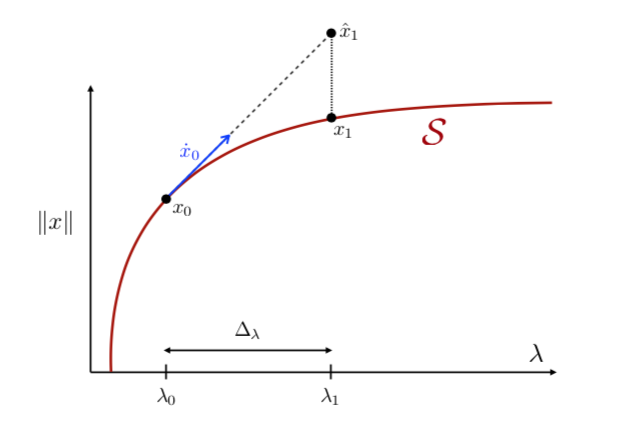
\includegraphics{image.png}

imagen tomada de la notas de Jean-Philippe Lessard

    El predictor se obtiene asumiendo que en la solución
\((x_0, \lambda_0)\) la matriz jacobiaba
\(\mathcal{D}_{x}F(x_0, \lambda_0)\) es invertible. Por el teorema de
función implicíta que curva solución está localmete parámetrizada por
\(\lambda\)

\[\dfrac{\partial}{\partial \lambda} F(x , \lambda) = 0 \Longrightarrow \mathcal{D}_{x}F(x_0, \lambda_0) \dfrac{d x}{\lambda}(\lambda)  + \dfrac{\partial F}{\partial \lambda} (x , \lambda) = 0  \Longrightarrow  \dfrac{d x}{d \lambda}(\lambda)  =  -\left( \mathcal{D}_{x}F(x_0, \lambda_0) \right)^{-1} \dfrac{\partial F}{\partial  \lambda} (x , \lambda) \]

El vector tangente a \((x_0, \lambda_0)\) se obtiene
\(\dot{x}_{0} = \dfrac{d x}{d \lambda}(\lambda_0)\), es decir
\[\dot{x}_{0} = -\left( \mathcal{D}_{x}F(x_0, \lambda_0) \right)^{-1} \dfrac{\partial F}{\partial  \lambda} (x_0 , \lambda_0) \]

Ya que tenemos el vector tangente, el predictor se define por
\[\hat{x_1} = x_0 + \Delta_{\lambda}\dot{x}_0\]

Después corregimos el predictor usando el método de Newton

\[x_1^{(0)} = \hat{x_1}, \quad  x_1^{(n+1)} = -\left( \mathcal{D}_{x}F(x_1^{(n)}, \lambda_1) \right)^{-1} F \left(x_1^{(n)} , \lambda_{1} \right)\]

    Algunas veces resulta mas natural parametrizar la rama solución por
\emph{longitud de arco} o \emph{pseudolongitud de arco} esto cuando la
curva no se puede parametrizar localmente por \(\lambda\), es decir
donde la matrix Jacobiana es singular

    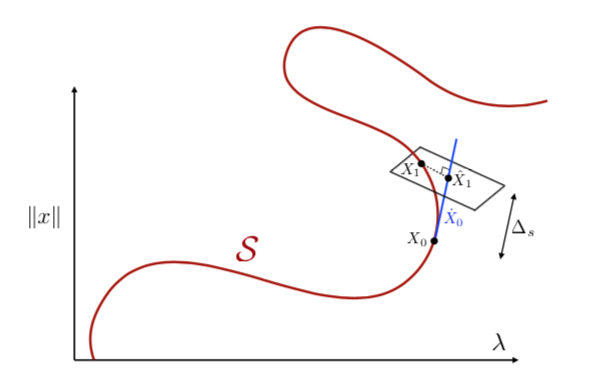
\includegraphics{image2.png}

    En el algoritmo de continuación de pseudolongitud de arco el valor del
parámetro ya no es fijo y en su lugar se deja como una variable. Si
tomamos \(X = (x, \lambda)\) y el problema \(F(X) = 0\) tal que
\(F:\mathbb{R}^{n+1} \longrightarrow \mathbb{R}^{n}\) y procediento de
manera análoga como antes. El proceso comienza con una solución \(X_0\)
dada con la que se genera un predictor, calculamos primero un vector
tangente unitario a la curva en \(X_0\), esto es

\[\mathcal{D}_{x}F(X_0)\dot{X}_0 = \left[ \mathcal{D}_{x}F(\overline{x}_0, \overline{\lambda}_0)  \dfrac{\partial F}{\partial  \lambda} (x_0 , \lambda_0) \right]\dot{X}_0 = 0 \in \mathbb{R}^n \]

Ahora fijamos un parametro de pseudolongitud de arco \(\Delta_{s} > 0\)
entonces definimos al predictor como

\[\hat{X_1} = \overline{X}_0 + \Delta_{s} \dot{X}_0 \in \mathbb{R}^{n+1}\]

Una vez que se tiene predictor, corregimos hacia el conjunto
\(\mathcal{S}\) en el hiperplano
\(E(X) := (X - \hat{E_1})\cdot \dot{X}_0 = 0\) perpendicular al vector
tangente \(\dot{X}_0\) que contiene el predictor \(X_1\). Como en el
caso anterior aplicamos el método de Newton pero a la función

\begin{equation}
X \mapsto \begin{bmatrix}
           E(X) \\
           F(X)
         \end{bmatrix}  
\end{equation}

Los algoritmos mencionados anteriormente no cubren el caso de
bifurcaciones de soluciones, pitchfork, puntos de bifurcación,
bifurcaciones de Hopf, etc.

    \hypertarget{un-ejemplo}{%
\paragraph{Un ejemplo}\label{un-ejemplo}}

Consideremos el modelo de circulación atmosferica introducido por Lorenz

\[  \left\{
\begin{array}{ll}
      x'_1 = - \alpha x_1 -x_2^2 - x_3^2 + \alpha\lambda & \\
      x'_2 = - x_2 - x_1x_2 - \beta x_1x_3 + \gamma & \\
      x'_3 = - x_3 - \beta x_1x_2 - x_1x_3 &
\end{array} 
\right.\]

Para el caso particular de \(\alpha = 0.25\) , \(\beta = 4\) y
\(\gamma = 0.5\) tenemos

\[ F(x, \lambda) =  \left(
\begin{array}{l}
      - \frac{1}{4} x_1 -x_2^2 - x_3^2 + \frac{\lambda}{4} \\
      - x_2 + x_1x_2 - 4 x_1x_3 + \frac{1}{2} \\
      - x_3 + 4 x_1x_2 + x_1x_3 
\end{array} 
\right) = 0\]

    \begin{Verbatim}[commandchars=\\\{\}]
{\color{incolor}In [{\color{incolor}18}]:} \PY{k}{using} \PY{n}{SymPy}
         
         \PY{n}{x1}\PY{p}{,} \PY{n}{x2}\PY{p}{,} \PY{n}{x3}\PY{p}{,} \PY{n}{l} \PY{o}{=} \PY{n}{symbols}\PY{p}{(}\PY{l+s}{\PYZdq{}}\PY{l+s}{x}\PY{l+s}{1}\PY{l+s}{,}\PY{l+s}{ }\PY{l+s}{x}\PY{l+s}{2}\PY{l+s}{ }\PY{l+s}{,}\PY{l+s}{ }\PY{l+s}{x}\PY{l+s}{3}\PY{l+s}{ }\PY{l+s}{,}\PY{l+s}{ }\PY{l+s}{l}\PY{l+s}{\PYZdq{}}\PY{p}{,} \PY{n}{real}\PY{o}{=}\PY{k+kc}{true}\PY{p}{)}
         
         \PY{n}{b1}\PY{p}{,} \PY{n}{b2}\PY{p}{,} \PY{n}{b3}   \PY{o}{=} \PY{n}{symbols}\PY{p}{(}\PY{l+s}{\PYZdq{}}\PY{l+s}{b}\PY{l+s}{1}\PY{l+s}{,}\PY{l+s}{ }\PY{l+s}{b}\PY{l+s}{2}\PY{l+s}{,}\PY{l+s}{ }\PY{l+s}{b}\PY{l+s}{3}\PY{l+s}{\PYZdq{}}\PY{p}{,} \PY{n}{real}\PY{o}{=}\PY{k+kc}{true}\PY{p}{)}
         
         \PY{n}{c1}\PY{p}{,} \PY{n}{c2}\PY{p}{,} \PY{n}{c3}   \PY{o}{=} \PY{n}{symbols}\PY{p}{(}\PY{l+s}{\PYZdq{}}\PY{l+s}{c}\PY{l+s}{1}\PY{l+s}{,}\PY{l+s}{ }\PY{l+s}{c}\PY{l+s}{2}\PY{l+s}{,}\PY{l+s}{ }\PY{l+s}{c}\PY{l+s}{3}\PY{l+s}{\PYZdq{}}\PY{p}{,} \PY{n}{real}\PY{o}{=}\PY{k+kc}{true}\PY{p}{)}
\end{Verbatim}


\begin{Verbatim}[commandchars=\\\{\}]
{\color{outcolor}Out[{\color{outcolor}18}]:} (c1, c2, c3)
\end{Verbatim}
            
    \begin{Verbatim}[commandchars=\\\{\}]
{\color{incolor}In [{\color{incolor}11}]:} \PY{n}{ex} \PY{o}{=} \PY{n}{x1}\PY{o}{\PYZca{}}\PY{l+m+mi}{2}\PY{o}{*}\PY{n}{cos}\PY{p}{(}\PY{n}{x2}\PY{p}{)}
\end{Verbatim}

\texttt{\color{outcolor}Out[{\color{outcolor}11}]:}
    
    $$x_{1}^{2} \cos{\left (x_{2} \right )}$$

    

    \begin{Verbatim}[commandchars=\\\{\}]
{\color{incolor}In [{\color{incolor}12}]:} \PY{n}{Sym}\PY{p}{[}\PY{n}{diff}\PY{p}{(}\PY{n}{ex}\PY{p}{,}\PY{n}{v1}\PY{p}{,} \PY{n}{v2}\PY{p}{)} \PY{k}{for} \PY{n}{v1} \PY{k+kp}{in} \PY{p}{[}\PY{n}{x1}\PY{p}{,}\PY{n}{x2}\PY{p}{]}\PY{p}{,} \PY{n}{v2} \PY{k+kp}{in} \PY{p}{[}\PY{n}{x1}\PY{p}{,}\PY{n}{x2}\PY{p}{]}\PY{p}{]}
\end{Verbatim}

\texttt{\color{outcolor}Out[{\color{outcolor}12}]:}
    
    \begin{bmatrix}2 \cos{\left (x_{2} \right )}&- 2 x_{1} \sin{\left (x_{2} \right )}\\- 2 x_{1} \sin{\left (x_{2} \right )}&- x_{1}^{2} \cos{\left (x_{2} \right )}\end{bmatrix}

    

    \begin{Verbatim}[commandchars=\\\{\}]
{\color{incolor}In [{\color{incolor}13}]:} \PY{n}{Ff} \PY{o}{=} \PY{p}{(}\PY{o}{\PYZhy{}} \PY{p}{(}\PY{l+m+mi}{1}\PY{o}{/}\PY{l+m+mi}{4}\PY{p}{)}\PY{o}{*}\PY{n}{x1} \PY{o}{\PYZhy{}}\PY{n}{x2}\PY{o}{\PYZca{}}\PY{l+m+mi}{2} \PY{o}{\PYZhy{}} \PY{n}{x3}\PY{o}{\PYZca{}}\PY{l+m+mi}{2} \PY{o}{+} \PY{l+m+mf}{0.25}\PY{o}{*}\PY{n}{l}\PY{p}{,}  \PY{o}{\PYZhy{}} \PY{n}{x2} \PY{o}{+} \PY{n}{x1}\PY{o}{*}\PY{n}{x2} \PY{o}{\PYZhy{}} \PY{l+m+mi}{4}\PY{o}{*}\PY{n}{x1}\PY{o}{*}\PY{n}{x3} \PY{o}{+} \PY{l+m+mf}{0.5}\PY{p}{,} \PY{o}{\PYZhy{}} \PY{n}{x3} \PY{o}{+} \PY{l+m+mi}{4}\PY{o}{*}\PY{n}{x1}\PY{o}{*}\PY{n}{x2} \PY{o}{+} \PY{n}{x1}\PY{o}{*}\PY{n}{x3}\PY{p}{)}
\end{Verbatim}


\begin{Verbatim}[commandchars=\\\{\}]
{\color{outcolor}Out[{\color{outcolor}13}]:} (0.25*l - 0.25*x1 - x2\^{}2 - x3\^{}2, x1*x2 - 4*x1*x3 - x2 + 0.5, 4*x1*x2 + x1*x3 - x3)
\end{Verbatim}
            
    \begin{Verbatim}[commandchars=\\\{\}]
{\color{incolor}In [{\color{incolor}14}]:} \PY{n}{Sym}\PY{p}{[}\PY{n}{Ff}\PY{p}{[}\PY{n}{i}\PY{p}{]} \PY{k}{for} \PY{n}{i} \PY{k+kp}{in} \PY{p}{[}\PY{l+m+mi}{1}\PY{p}{,}\PY{l+m+mi}{2}\PY{p}{,}\PY{l+m+mi}{3}\PY{p}{]}\PY{p}{]}
\end{Verbatim}

\texttt{\color{outcolor}Out[{\color{outcolor}14}]:}
    
    \begin{bmatrix}0.25 l - 0.25 x_{1} - x_{2}^{2} - x_{3}^{2}\\x_{1} x_{2} - 4 x_{1} x_{3} - x_{2} + 0.5\\4 x_{1} x_{2} + x_{1} x_{3} - x_{3}\end{bmatrix}

    

    \begin{Verbatim}[commandchars=\\\{\}]
{\color{incolor}In [{\color{incolor}15}]:} \PY{n}{DxF} \PY{o}{=} \PY{n}{Sym}\PY{p}{[}\PY{n}{diff}\PY{p}{(}\PY{n}{Ff}\PY{p}{[}\PY{n}{v1}\PY{p}{]}\PY{p}{,} \PY{n}{v2}\PY{p}{)} \PY{k}{for} \PY{n}{v1} \PY{k+kp}{in} \PY{p}{[}\PY{l+m+mi}{1}\PY{p}{,}\PY{l+m+mi}{2}\PY{p}{,}\PY{l+m+mi}{3}\PY{p}{]}\PY{p}{,} \PY{n}{v2} \PY{k+kp}{in} \PY{p}{[}\PY{n}{x1}\PY{p}{,}\PY{n}{x2}\PY{p}{,}\PY{n}{x3}\PY{p}{]}\PY{p}{]}
\end{Verbatim}

\texttt{\color{outcolor}Out[{\color{outcolor}15}]:}
    
    \begin{bmatrix}-0.25&- 2 x_{2}&- 2 x_{3}\\x_{2} - 4 x_{3}&x_{1} - 1&- 4 x_{1}\\4 x_{2} + x_{3}&4 x_{1}&x_{1} - 1\end{bmatrix}

    

    Deseamos utilizar el Teorema de la aproximación del radio de polinomios
para probar la existencia de un segmento de soluciones en el conjunto de
soluciones en el conjunto
\(\mathcal{S} = \{(x,\lambda) \in \mathbb{R}^4 \vert F(x,\lambda) = 0\}\)
y consideremos el conjuntos de los predictores
\[\bar{x}_s = (1 - s)\bar{x}_0 + s\bar{x}_1 \text{ y } \bar{\lambda}_s = (1 - s)\bar{\lambda}_0 + s\bar{\lambda}_1\]
Para \(s \in [0,1]\), además definimos
\(\Delta\bar{x} := \bar{x}_1 - \bar{x}_0\) y
\(\Delta\bar{\lambda} := \bar{\lambda}_1 - \bar{\lambda}_0\)

    Ahora calculemos la cotas del teorema de la aproximación del radio
polinimial del cual tenemos

\begin{itemize}
\tightlist
\item
  \(\vert \vert AF(x_{s}, \lambda_{}) \vert \vert_{X} \leq \mathbf{Y_0} \quad \forall s \in [0,1]\)
\item
  \(\vert \vert I - AA^{\dagger} \vert \vert_{B(X,X)} \leq \mathbf{Z_0}\)
\item
  \(\vert \vert A[\mathcal{D}_xF(\bar{x}_0, \lambda_0) - A^{\dagger}] \vert \vert_{B(X,X)} \leq \mathbf{Z_1}\)
\item
  \(\vert \vert A[\mathcal{D}_xF(\bar{x}_s + b, \lambda_s) - \mathcal{D}_xF(\bar{x}_0, \lambda_0)] \vert \vert_{B(X,X)} \leq \mathbf{Z_2}(r) \quad \forall \in B_r(0) \text{ y } \forall s \in [0,1]\)
\end{itemize}

Comencemos por calcular \(\mathbf{Y_0}\) consideremos la expansión:

\[F(\bar{x}_s, \lambda_s) = F(\bar{x}_0, \lambda_0) + \left[ \mathcal{D}_x F(\bar{x}_0, \lambda_0) \quad \dfrac{\partial F}{\partial \lambda} (\bar{x}_0, \lambda_0) \right]\begin{pmatrix}
           \Delta \bar{x} \\
           \Delta \lambda  
         \end{pmatrix} s + \dfrac{1}{2} \left( \dfrac{\partial ^2}{\partial s^2}  F(\bar{x}_s, \lambda_s)\bigg\lvert_{s=0} \right) s^2  +h.o.t\]

Aplicando el operador \(A\), tenemos:
\[\vert \vert AF(\bar{x}_s, \lambda_s)\vert \vert_{X} \leq \vert \vert AF(\bar{x}_0, \lambda_0)\vert \vert_{X}  + \vert \vert Ay_1 \vert \vert_{X} + \vert \vert Ay_2\vert \vert_{X} + \delta \]

\[y_2 = \begin{pmatrix}
           -(\Delta \bar{x})_2 ^2 - (\Delta \bar{x})_3 ^2  \\
           (\Delta \bar{x})_1(\Delta \bar{x})_2 - 4(\Delta \bar{x})_1(\Delta \bar{x})_3  \\
           4(\Delta \bar{x})_1(\Delta \bar{x})_2 + (\Delta \bar{x})_1(\Delta \bar{x})_3  
         \end{pmatrix} \]

A continuación calcularemos \(y_1\), primero calculemos
\(\left[ \mathcal{D}_x F(\bar{x}_0, \lambda_0) \quad \dfrac{\partial F}{\partial \lambda} (\bar{x}_0, \lambda_0) \right]\)

    \begin{Verbatim}[commandchars=\\\{\}]
{\color{incolor}In [{\color{incolor}16}]:} \PY{n}{DxFext} \PY{o}{=} \PY{n}{Sym}\PY{p}{[}\PY{n}{diff}\PY{p}{(}\PY{n}{Ff}\PY{p}{[}\PY{n}{v1}\PY{p}{]}\PY{p}{,} \PY{n}{v2}\PY{p}{)} \PY{k}{for} \PY{n}{v1} \PY{k+kp}{in} \PY{p}{[}\PY{l+m+mi}{1}\PY{p}{,}\PY{l+m+mi}{2}\PY{p}{,}\PY{l+m+mi}{3}\PY{p}{]}\PY{p}{,} \PY{n}{v2} \PY{k+kp}{in} \PY{p}{[}\PY{n}{x1}\PY{p}{,}\PY{n}{x2}\PY{p}{,}\PY{n}{x3}\PY{p}{,}\PY{n}{l}\PY{p}{]}\PY{p}{]}
\end{Verbatim}

\texttt{\color{outcolor}Out[{\color{outcolor}16}]:}
    
    \begin{bmatrix}-0.25&- 2 x_{2}&- 2 x_{3}&0.25\\x_{2} - 4 x_{3}&x_{1} - 1&- 4 x_{1}&0\\4 x_{2} + x_{3}&4 x_{1}&x_{1} - 1&0\end{bmatrix}

    

    \begin{Verbatim}[commandchars=\\\{\}]
{\color{incolor}In [{\color{incolor}44}]:} \PY{n}{Dx1}\PY{p}{,} \PY{n}{Dx2}\PY{p}{,} \PY{n}{Dx3}\PY{p}{,} \PY{n}{Dl} \PY{o}{=} \PY{n}{symbols}\PY{p}{(}\PY{l+s}{\PYZdq{}}\PY{l+s}{D}\PY{l+s}{x}\PY{l+s}{1}\PY{l+s}{,}\PY{l+s}{ }\PY{l+s}{D}\PY{l+s}{x}\PY{l+s}{2}\PY{l+s}{ }\PY{l+s}{,}\PY{l+s}{ }\PY{l+s}{D}\PY{l+s}{x}\PY{l+s}{3}\PY{l+s}{ }\PY{l+s}{,}\PY{l+s}{ }\PY{l+s}{D}\PY{l+s}{l}\PY{l+s}{\PYZdq{}}\PY{p}{,} \PY{n}{real}\PY{o}{=}\PY{k+kc}{true}\PY{p}{)}
         \PY{n}{Dxλ} \PY{o}{=}  \PY{n}{Sym}\PY{p}{[} \PY{n}{Dx1}\PY{p}{,} \PY{n}{Dx2}\PY{p}{,} \PY{n}{Dx3}\PY{p}{,} \PY{n}{Dl}\PY{p}{]}
\end{Verbatim}

\texttt{\color{outcolor}Out[{\color{outcolor}44}]:}
    
    \begin{bmatrix}Dx_{1}\\Dx_{2}\\Dx_{3}\\Dl\end{bmatrix}

    

    \begin{Verbatim}[commandchars=\\\{\}]
{\color{incolor}In [{\color{incolor}47}]:} \PY{n}{FFS} \PY{o}{=} \PY{n}{DxFext}\PY{o}{*}\PY{n}{Dxλ}
\end{Verbatim}

\texttt{\color{outcolor}Out[{\color{outcolor}47}]:}
    
    \begin{bmatrix}0.25 Dl - 0.25 Dx_{1} - 2 Dx_{2} x_{2} - 2 Dx_{3} x_{3}\\Dx_{1} \left(x_{2} - 4 x_{3}\right) + Dx_{2} \left(x_{1} - 1\right) - 4 Dx_{3} x_{1}\\Dx_{1} \left(4 x_{2} + x_{3}\right) + 4 Dx_{2} x_{1} + Dx_{3} \left(x_{1} - 1\right)\end{bmatrix}

    

    \begin{Verbatim}[commandchars=\\\{\}]
{\color{incolor}In [{\color{incolor}37}]:} \PY{k}{function} \PY{n}{f!}\PY{p}{(}\PY{n}{F}\PY{p}{,}\PY{n}{x}\PY{p}{)}
             \PY{n}{λ} \PY{o}{=} \PY{l+m+mf}{0.85}
             \PY{n}{F}\PY{p}{[}\PY{l+m+mi}{1}\PY{p}{]} \PY{o}{=} \PY{o}{\PYZhy{}}\PY{l+m+mf}{0.25}\PY{o}{*}\PY{n}{x}\PY{p}{[}\PY{l+m+mi}{1}\PY{p}{]} \PY{o}{\PYZhy{}}\PY{n}{x}\PY{p}{[}\PY{l+m+mi}{2}\PY{p}{]}\PY{o}{\PYZca{}}\PY{l+m+mi}{2} \PY{o}{\PYZhy{}} \PY{n}{x}\PY{p}{[}\PY{l+m+mi}{3}\PY{p}{]}\PY{o}{\PYZca{}}\PY{l+m+mi}{2} \PY{o}{+} \PY{l+m+mf}{0.25}\PY{o}{*}\PY{n}{λ}
             \PY{n}{F}\PY{p}{[}\PY{l+m+mi}{2}\PY{p}{]} \PY{o}{=} \PY{o}{\PYZhy{}}\PY{n}{x}\PY{p}{[}\PY{l+m+mi}{2}\PY{p}{]} \PY{o}{+} \PY{n}{x}\PY{p}{[}\PY{l+m+mi}{1}\PY{p}{]}\PY{o}{*}\PY{n}{x}\PY{p}{[}\PY{l+m+mi}{2}\PY{p}{]} \PY{o}{\PYZhy{}} \PY{l+m+mi}{4}\PY{o}{*}\PY{n}{x}\PY{p}{[}\PY{l+m+mi}{1}\PY{p}{]}\PY{n}{x}\PY{p}{[}\PY{l+m+mi}{3}\PY{p}{]} \PY{o}{+} \PY{l+m+mf}{0.5}
             \PY{n}{F}\PY{p}{[}\PY{l+m+mi}{3}\PY{p}{]} \PY{o}{=} \PY{o}{\PYZhy{}}\PY{n}{x}\PY{p}{[}\PY{l+m+mi}{3}\PY{p}{]} \PY{o}{+} \PY{l+m+mi}{4}\PY{o}{*}\PY{n}{x}\PY{p}{[}\PY{l+m+mi}{1}\PY{p}{]}\PY{o}{*}\PY{n}{x}\PY{p}{[}\PY{l+m+mi}{2}\PY{p}{]} \PY{o}{+} \PY{n}{x}\PY{p}{[}\PY{l+m+mi}{1}\PY{p}{]}\PY{n}{x}\PY{p}{[}\PY{l+m+mi}{3}\PY{p}{]} 
         \PY{k}{end}
         
         \PY{k}{function} \PY{n}{j!}\PY{p}{(}\PY{n}{J}\PY{p}{,}\PY{n}{x}\PY{p}{)}
             \PY{n}{J}\PY{p}{[}\PY{l+m+mi}{1}\PY{p}{,} \PY{l+m+mi}{1}\PY{p}{]} \PY{o}{=} \PY{o}{\PYZhy{}}\PY{l+m+mf}{0.25}
             \PY{n}{J}\PY{p}{[}\PY{l+m+mi}{1}\PY{p}{,} \PY{l+m+mi}{2}\PY{p}{]} \PY{o}{=} \PY{o}{\PYZhy{}}\PY{l+m+mi}{2}\PY{o}{*}\PY{n}{x}\PY{p}{[}\PY{l+m+mi}{2}\PY{p}{]}
             \PY{n}{J}\PY{p}{[}\PY{l+m+mi}{1}\PY{p}{,} \PY{l+m+mi}{3}\PY{p}{]} \PY{o}{=} \PY{o}{\PYZhy{}}\PY{l+m+mi}{2}\PY{o}{*}\PY{n}{x}\PY{p}{[}\PY{l+m+mi}{3}\PY{p}{]}
             \PY{n}{J}\PY{p}{[}\PY{l+m+mi}{2}\PY{p}{,} \PY{l+m+mi}{1}\PY{p}{]} \PY{o}{=} \PY{n}{x}\PY{p}{[}\PY{l+m+mi}{2}\PY{p}{]} \PY{o}{\PYZhy{}}\PY{l+m+mi}{4}\PY{o}{*}\PY{n}{x}\PY{p}{[}\PY{l+m+mi}{3}\PY{p}{]}
             \PY{n}{J}\PY{p}{[}\PY{l+m+mi}{2}\PY{p}{,} \PY{l+m+mi}{2}\PY{p}{]} \PY{o}{=} \PY{o}{\PYZhy{}}\PY{l+m+mi}{1} \PY{o}{+} \PY{n}{x}\PY{p}{[}\PY{l+m+mi}{1}\PY{p}{]}
             \PY{n}{J}\PY{p}{[}\PY{l+m+mi}{2}\PY{p}{,} \PY{l+m+mi}{3}\PY{p}{]} \PY{o}{=} \PY{o}{\PYZhy{}}\PY{l+m+mi}{4}\PY{o}{*}\PY{n}{x}\PY{p}{[}\PY{l+m+mi}{1}\PY{p}{]}
             \PY{n}{J}\PY{p}{[}\PY{l+m+mi}{3}\PY{p}{,} \PY{l+m+mi}{1}\PY{p}{]} \PY{o}{=} \PY{l+m+mi}{4}\PY{o}{*}\PY{n}{x}\PY{p}{[}\PY{l+m+mi}{2}\PY{p}{]} \PY{o}{+} \PY{n}{x}\PY{p}{[}\PY{l+m+mi}{3}\PY{p}{]}
             \PY{n}{J}\PY{p}{[}\PY{l+m+mi}{3}\PY{p}{,} \PY{l+m+mi}{2}\PY{p}{]} \PY{o}{=} \PY{l+m+mi}{4}\PY{o}{*}\PY{n}{x}\PY{p}{[}\PY{l+m+mi}{1}\PY{p}{]}
             \PY{n}{J}\PY{p}{[}\PY{l+m+mi}{3}\PY{p}{,} \PY{l+m+mi}{3}\PY{p}{]} \PY{o}{=} \PY{o}{\PYZhy{}}\PY{l+m+mi}{1} \PY{o}{+} \PY{n}{x}\PY{p}{[}\PY{l+m+mi}{1}\PY{p}{]}
             
         \PY{k}{end}
\end{Verbatim}


\begin{Verbatim}[commandchars=\\\{\}]
{\color{outcolor}Out[{\color{outcolor}37}]:} j! (generic function with 1 method)
\end{Verbatim}
            
    \begin{Verbatim}[commandchars=\\\{\}]
{\color{incolor}In [{\color{incolor}35}]:} \PY{n}{xbar0} \PY{o}{=} \PY{n}{nlsolve}\PY{p}{(}\PY{n}{f!}\PY{p}{,} \PY{p}{[} \PY{o}{\PYZhy{}}\PY{l+m+mf}{0.05}\PY{p}{;} \PY{l+m+mf}{0.4}\PY{p}{;} \PY{o}{\PYZhy{}}\PY{l+m+mf}{0.09}\PY{p}{]}\PY{p}{,} \PY{n}{autodiff} \PY{o}{=} \PY{o}{:}\PY{n}{forward}\PY{p}{,} \PY{n}{ftol}\PY{o}{=}\PY{l+m+mf}{1.0e\PYZhy{}18}\PY{p}{,} \PY{n}{iterations} \PY{o}{=}\PY{l+m+mi}{100}\PY{p}{)}
\end{Verbatim}


\begin{Verbatim}[commandchars=\\\{\}]
{\color{outcolor}Out[{\color{outcolor}35}]:} Results of Nonlinear Solver Algorithm
          * Algorithm: Trust-region with dogleg and autoscaling
          * Starting Point: [-0.05, 0.4, -0.09]
          * Zero: [-0.0565519, 0.452496, -0.0968792]
          * Inf-norm of residuals: 0.000000
          * Iterations: 100
          * Convergence: false
            * |x - x'| < 0.0e+00: false
            * |f(x)| < 1.0e-18: false
          * Function Calls (f): 15
          * Jacobian Calls (df/dx): 9
\end{Verbatim}
            
    \begin{Verbatim}[commandchars=\\\{\}]
{\color{incolor}In [{\color{incolor}38}]:} \PY{n}{xbar1} \PY{o}{=} \PY{n}{nlsolve}\PY{p}{(}\PY{n}{f!}\PY{p}{,} \PY{p}{[} \PY{o}{\PYZhy{}}\PY{l+m+mf}{0.05}\PY{p}{;} \PY{l+m+mf}{0.4}\PY{p}{;} \PY{l+m+mf}{0.09}\PY{p}{]}\PY{p}{,} \PY{n}{autodiff} \PY{o}{=} \PY{o}{:}\PY{n}{forward}\PY{p}{,}\PY{n}{ftol}\PY{o}{=}\PY{l+m+mf}{1.0e\PYZhy{}18}\PY{p}{,} \PY{n}{iterations} \PY{o}{=}\PY{l+m+mi}{100}\PY{p}{)}
\end{Verbatim}


\begin{Verbatim}[commandchars=\\\{\}]
{\color{outcolor}Out[{\color{outcolor}38}]:} Results of Nonlinear Solver Algorithm
          * Algorithm: Trust-region with dogleg and autoscaling
          * Starting Point: [-0.05, 0.4, 0.09]
          * Zero: [-0.0435055, 0.466189, -0.0777448]
          * Inf-norm of residuals: 0.000000
          * Iterations: 100
          * Convergence: false
            * |x - x'| < 0.0e+00: false
            * |f(x)| < 1.0e-18: false
          * Function Calls (f): 8
          * Jacobian Calls (df/dx): 8
\end{Verbatim}
            
    \begin{Verbatim}[commandchars=\\\{\}]
{\color{incolor}In [{\color{incolor}36}]:} \PY{n}{xbar0}\PY{o}{.}\PY{n}{zero}
\end{Verbatim}


\begin{Verbatim}[commandchars=\\\{\}]
{\color{outcolor}Out[{\color{outcolor}36}]:} 3-element Array\{Float64,1\}:
          -0.0565519
           0.452496 
          -0.0968792
\end{Verbatim}
            
    \begin{Verbatim}[commandchars=\\\{\}]
{\color{incolor}In [{\color{incolor}39}]:} \PY{n}{xbar1}\PY{o}{.}\PY{n}{zero}
\end{Verbatim}


\begin{Verbatim}[commandchars=\\\{\}]
{\color{outcolor}Out[{\color{outcolor}39}]:} 3-element Array\{Float64,1\}:
          -0.0435055
           0.466189 
          -0.0777448
\end{Verbatim}
            
    \begin{Verbatim}[commandchars=\\\{\}]
{\color{incolor}In [{\color{incolor}42}]:} \PY{n}{Δx} \PY{o}{=} \PY{n}{xbar1}\PY{o}{.}\PY{n}{zero} \PY{o}{\PYZhy{}} \PY{n}{xbar0}\PY{o}{.}\PY{n}{zero}
\end{Verbatim}


\begin{Verbatim}[commandchars=\\\{\}]
{\color{outcolor}Out[{\color{outcolor}42}]:} 3-element Array\{Float64,1\}:
          0.0130464
          0.0136932
          0.0191344
\end{Verbatim}
            
    \begin{Verbatim}[commandchars=\\\{\}]
{\color{incolor}In [{\color{incolor}43}]:} \PY{n}{Δλ} \PY{o}{=} \PY{l+m+mf}{0.05}
\end{Verbatim}


\begin{Verbatim}[commandchars=\\\{\}]
{\color{outcolor}Out[{\color{outcolor}43}]:} 0.05
\end{Verbatim}
            
    Calculemos el operador
\(A^{\dagger} \approx \mathcal{D}F(\bar{x}_0, \lambda_0)\)

    \begin{Verbatim}[commandchars=\\\{\}]
{\color{incolor}In [{\color{incolor}49}]:} \PY{k}{function} \PY{n}{F}\PY{p}{(}\PY{n}{x}\PY{o}{::}\PY{k+kt}{Vector}\PY{p}{)}
             \PY{n}{λ} \PY{o}{=} \PY{l+m+mf}{0.8}
             \PY{n}{x1} \PY{o}{=} \PY{o}{\PYZhy{}}\PY{l+m+mf}{0.25}\PY{o}{*}\PY{n}{x}\PY{p}{[}\PY{l+m+mi}{1}\PY{p}{]} \PY{o}{\PYZhy{}}\PY{n}{x}\PY{p}{[}\PY{l+m+mi}{2}\PY{p}{]}\PY{o}{\PYZca{}}\PY{l+m+mi}{2} \PY{o}{\PYZhy{}} \PY{n}{x}\PY{p}{[}\PY{l+m+mi}{3}\PY{p}{]}\PY{o}{\PYZca{}}\PY{l+m+mi}{2} \PY{o}{+} \PY{l+m+mf}{0.25}\PY{o}{*}\PY{n}{λ}
             \PY{n}{x2} \PY{o}{=} \PY{o}{\PYZhy{}}\PY{n}{x}\PY{p}{[}\PY{l+m+mi}{2}\PY{p}{]} \PY{o}{+} \PY{n}{x}\PY{p}{[}\PY{l+m+mi}{1}\PY{p}{]}\PY{o}{*}\PY{n}{x}\PY{p}{[}\PY{l+m+mi}{2}\PY{p}{]} \PY{o}{\PYZhy{}} \PY{l+m+mi}{4}\PY{o}{*}\PY{n}{x}\PY{p}{[}\PY{l+m+mi}{1}\PY{p}{]}\PY{n}{x}\PY{p}{[}\PY{l+m+mi}{3}\PY{p}{]} \PY{o}{+} \PY{l+m+mf}{0.5}
             \PY{n}{x3} \PY{o}{=} \PY{o}{\PYZhy{}}\PY{n}{x}\PY{p}{[}\PY{l+m+mi}{3}\PY{p}{]} \PY{o}{+} \PY{l+m+mi}{4}\PY{o}{*}\PY{n}{x}\PY{p}{[}\PY{l+m+mi}{1}\PY{p}{]}\PY{o}{*}\PY{n}{x}\PY{p}{[}\PY{l+m+mi}{2}\PY{p}{]} \PY{o}{+} \PY{n}{x}\PY{p}{[}\PY{l+m+mi}{1}\PY{p}{]}\PY{n}{x}\PY{p}{[}\PY{l+m+mi}{3}\PY{p}{]} 
             \PY{k}{return} \PY{p}{[}\PY{n}{x1}\PY{p}{,} \PY{n}{x2}\PY{p}{,} \PY{n}{x3}\PY{p}{]}
         \PY{k}{end} 
         \PY{n}{DF} \PY{o}{=} \PY{n}{x} \PY{o}{\PYZhy{}}\PY{o}{\PYZgt{}} \PY{n}{ForwardDiff}\PY{o}{.}\PY{n}{jacobian}\PY{p}{(}\PY{n}{F}\PY{p}{,} \PY{n}{x}\PY{p}{)}
\end{Verbatim}


\begin{Verbatim}[commandchars=\\\{\}]
{\color{outcolor}Out[{\color{outcolor}49}]:} (::\#11) (generic function with 1 method)
\end{Verbatim}
            
    \begin{Verbatim}[commandchars=\\\{\}]
{\color{incolor}In [{\color{incolor}50}]:} \PY{n}{Adaga} \PY{o}{=} \PY{n}{DF}\PY{p}{(}\PY{n}{xbar0}\PY{o}{.}\PY{n}{zero}\PY{p}{)}
\end{Verbatim}


\begin{Verbatim}[commandchars=\\\{\}]
{\color{outcolor}Out[{\color{outcolor}50}]:} 3×3 Array\{Float64,2\}:
          -0.25      -0.904991   0.193758
           0.840013  -1.05655    0.226207
           1.7131    -0.226207  -1.05655 
\end{Verbatim}
            
    \begin{Verbatim}[commandchars=\\\{\}]
{\color{incolor}In [{\color{incolor}51}]:} \PY{n}{A} \PY{o}{=} \PY{n}{inv}\PY{p}{(}\PY{n}{Adaga}\PY{p}{)}
\end{Verbatim}


\begin{Verbatim}[commandchars=\\\{\}]
{\color{outcolor}Out[{\color{outcolor}51}]:} 3×3 Array\{Float64,2\}:
          -1.03144  0.883486    2.22045e-16
          -1.12647  0.0598917  -0.193758   
          -1.43122  1.41967    -0.904991   
\end{Verbatim}
            
    \begin{Verbatim}[commandchars=\\\{\}]
{\color{incolor}In [{\color{incolor}52}]:} \PY{n}{y1} \PY{o}{=} \PY{n}{A}\PY{o}{*}\PY{n}{F}\PY{p}{(}\PY{n}{xbar0}\PY{o}{.}\PY{n}{zero}\PY{p}{)}
\end{Verbatim}


\begin{Verbatim}[commandchars=\\\{\}]
{\color{outcolor}Out[{\color{outcolor}52}]:} 3-element Array\{Float64,1\}:
          -2.86283e-17
          -3.12659e-17
          -3.97242e-17
\end{Verbatim}
            
    \begin{Verbatim}[commandchars=\\\{\}]
{\color{incolor}In [{\color{incolor}53}]:} \PY{n}{y1max} \PY{o}{=} \PY{n}{maximum}\PY{p}{(}\PY{n}{abs}\PY{o}{.}\PY{p}{(}\PY{n}{y1}\PY{p}{)}\PY{p}{)}
\end{Verbatim}


\begin{Verbatim}[commandchars=\\\{\}]
{\color{outcolor}Out[{\color{outcolor}53}]:} 3.9724234750621873e-17
\end{Verbatim}
            
    \begin{Verbatim}[commandchars=\\\{\}]
{\color{incolor}In [{\color{incolor}54}]:} \PY{n}{a} \PY{o}{=}\PY{p}{[}\PY{n}{Adaga}\PY{p}{[}\PY{l+m+mi}{1}\PY{p}{]} \PY{n}{Adaga}\PY{p}{[}\PY{l+m+mi}{4}\PY{p}{]} \PY{n}{Adaga}\PY{p}{[}\PY{l+m+mi}{7}\PY{p}{]} \PY{l+m+mf}{0.25}\PY{p}{;} \PY{n}{Adaga}\PY{p}{[}\PY{l+m+mi}{2}\PY{p}{]} \PY{n}{Adaga}\PY{p}{[}\PY{l+m+mi}{5}\PY{p}{]} \PY{n}{Adaga}\PY{p}{[}\PY{l+m+mi}{8}\PY{p}{]} \PY{l+m+mf}{0.0}\PY{p}{;} \PY{n}{Adaga}\PY{p}{[}\PY{l+m+mi}{3}\PY{p}{]} \PY{n}{Adaga}\PY{p}{[}\PY{l+m+mi}{6}\PY{p}{]} \PY{n}{Adaga}\PY{p}{[}\PY{l+m+mi}{9}\PY{p}{]} \PY{l+m+mf}{0.0}\PY{p}{]}
\end{Verbatim}


\begin{Verbatim}[commandchars=\\\{\}]
{\color{outcolor}Out[{\color{outcolor}54}]:} 3×4 Array\{Float64,2\}:
          -0.25      -0.904991   0.193758  0.25
           0.840013  -1.05655    0.226207  0.0 
           1.7131    -0.226207  -1.05655   0.0 
\end{Verbatim}
            
    \begin{Verbatim}[commandchars=\\\{\}]
{\color{incolor}In [{\color{incolor}55}]:} \PY{n}{b} \PY{o}{=} \PY{p}{[}\PY{n}{Δx}\PY{p}{[}\PY{l+m+mi}{1}\PY{p}{]}\PY{p}{,} \PY{n}{Δx}\PY{p}{[}\PY{l+m+mi}{2}\PY{p}{]}\PY{p}{,} \PY{n}{Δx}\PY{p}{[}\PY{l+m+mi}{3}\PY{p}{]}\PY{p}{,} \PY{n}{Δλ}\PY{p}{]}
\end{Verbatim}


\begin{Verbatim}[commandchars=\\\{\}]
{\color{outcolor}Out[{\color{outcolor}55}]:} 4-element Array\{Float64,1\}:
          0.0130464
          0.0136932
          0.0191344
          0.05     
\end{Verbatim}
            
    \begin{Verbatim}[commandchars=\\\{\}]
{\color{incolor}In [{\color{incolor}56}]:} \PY{n}{y2} \PY{o}{=}  \PY{n}{a}\PY{o}{*}\PY{n}{b}
\end{Verbatim}


\begin{Verbatim}[commandchars=\\\{\}]
{\color{outcolor}Out[{\color{outcolor}56}]:} 3-element Array\{Float64,1\}:
           0.00055363 
           0.000819893
          -0.000964222
\end{Verbatim}
            
    \begin{Verbatim}[commandchars=\\\{\}]
{\color{incolor}In [{\color{incolor}57}]:} \PY{n}{subs}\PY{p}{(}\PY{n}{FF}\PY{p}{,} \PY{p}{(}\PY{n}{x1}\PY{p}{,} \PY{n}{xbar0}\PY{o}{.}\PY{n}{zero}\PY{p}{[}\PY{l+m+mi}{1}\PY{p}{]}\PY{p}{)}\PY{p}{,} \PY{p}{(}\PY{n}{x2}\PY{p}{,} \PY{n}{xbar0}\PY{o}{.}\PY{n}{zero}\PY{p}{[}\PY{l+m+mi}{2}\PY{p}{]}\PY{p}{)}\PY{p}{,} \PY{p}{(}\PY{n}{x3}\PY{p}{,} \PY{n}{xbar0}\PY{o}{.}\PY{n}{zero}\PY{p}{[}\PY{l+m+mi}{3}\PY{p}{]}\PY{p}{)}\PY{p}{)} \PY{o}{|\PYZgt{}} \PY{n}{float}
\end{Verbatim}


\begin{Verbatim}[commandchars=\\\{\}]
{\color{outcolor}Out[{\color{outcolor}57}]:} 3-element Array\{Float64,1\}:
           0.00055363 
           0.000819893
          -0.000964222
\end{Verbatim}
            
    \begin{Verbatim}[commandchars=\\\{\}]
{\color{incolor}In [{\color{incolor}58}]:} \PY{n}{y22} \PY{o}{=} \PY{n}{A}\PY{o}{*}\PY{n}{y2}
\end{Verbatim}


\begin{Verbatim}[commandchars=\\\{\}]
{\color{outcolor}Out[{\color{outcolor}58}]:} 3-element Array\{Float64,1\}:
           0.000153325
          -0.000387719
           0.00124423 
\end{Verbatim}
            
    \begin{Verbatim}[commandchars=\\\{\}]
{\color{incolor}In [{\color{incolor}59}]:} \PY{n}{y2max} \PY{o}{=} \PY{n}{maximum}\PY{p}{(}\PY{n}{abs}\PY{o}{.}\PY{p}{(}\PY{n}{y22}\PY{p}{)}\PY{p}{)}
\end{Verbatim}


\begin{Verbatim}[commandchars=\\\{\}]
{\color{outcolor}Out[{\color{outcolor}59}]:} 0.0012442255575526046
\end{Verbatim}
            
    \begin{Verbatim}[commandchars=\\\{\}]
{\color{incolor}In [{\color{incolor}60}]:} \PY{n}{y3} \PY{o}{=} \PY{p}{[}\PY{o}{\PYZhy{}}\PY{n}{Δx}\PY{p}{[}\PY{l+m+mi}{2}\PY{p}{]}\PY{o}{\PYZca{}}\PY{l+m+mi}{2} \PY{o}{\PYZhy{}} \PY{n}{Δx}\PY{p}{[}\PY{l+m+mi}{3}\PY{p}{]}\PY{o}{\PYZca{}}\PY{l+m+mi}{2}\PY{p}{,} \PY{n}{Δx}\PY{p}{[}\PY{l+m+mi}{1}\PY{p}{]}\PY{o}{*}\PY{n}{Δx}\PY{p}{[}\PY{l+m+mi}{2}\PY{p}{]} \PY{o}{\PYZhy{}} \PY{l+m+mi}{4}\PY{o}{*}\PY{n}{Δx}\PY{p}{[}\PY{l+m+mi}{1}\PY{p}{]}\PY{o}{*}\PY{n}{Δx}\PY{p}{[}\PY{l+m+mi}{3}\PY{p}{]}\PY{p}{,} \PY{l+m+mi}{4}\PY{o}{*}\PY{n}{Δx}\PY{p}{[}\PY{l+m+mi}{1}\PY{p}{]}\PY{o}{*}\PY{n}{Δx}\PY{p}{[}\PY{l+m+mi}{2}\PY{p}{]} \PY{o}{+} \PY{n}{Δx}\PY{p}{[}\PY{l+m+mi}{1}\PY{p}{]}\PY{o}{*}\PY{n}{Δx}\PY{p}{[}\PY{l+m+mi}{3}\PY{p}{]}\PY{p}{]}
\end{Verbatim}


\begin{Verbatim}[commandchars=\\\{\}]
{\color{outcolor}Out[{\color{outcolor}60}]:} 3-element Array\{Float64,1\}:
          -0.00055363 
          -0.000819893
           0.000964222
\end{Verbatim}
            
    \begin{Verbatim}[commandchars=\\\{\}]
{\color{incolor}In [{\color{incolor}61}]:} \PY{n}{y33} \PY{o}{=} \PY{n}{A}\PY{o}{*}\PY{n}{y3}
\end{Verbatim}


\begin{Verbatim}[commandchars=\\\{\}]
{\color{outcolor}Out[{\color{outcolor}61}]:} 3-element Array\{Float64,1\}:
          -0.000153325
           0.000387719
          -0.00124423 
\end{Verbatim}
            
    \begin{Verbatim}[commandchars=\\\{\}]
{\color{incolor}In [{\color{incolor}62}]:} \PY{n}{y3max} \PY{o}{=} \PY{n}{maximum}\PY{p}{(}\PY{n}{abs}\PY{o}{.}\PY{p}{(}\PY{n}{y33}\PY{p}{)}\PY{p}{)}
\end{Verbatim}


\begin{Verbatim}[commandchars=\\\{\}]
{\color{outcolor}Out[{\color{outcolor}62}]:} 0.001244225557552599
\end{Verbatim}
            
    \begin{Verbatim}[commandchars=\\\{\}]
{\color{incolor}In [{\color{incolor}63}]:} \PY{n}{Y0} \PY{o}{=} \PY{n}{y1max} \PY{o}{+} \PY{n}{y2max} \PY{o}{+} \PY{n}{y3max}
\end{Verbatim}


\begin{Verbatim}[commandchars=\\\{\}]
{\color{outcolor}Out[{\color{outcolor}63}]:} 0.002488451115105243
\end{Verbatim}
            
    \(\mathbf{Y_0}= 0.002488451115105243\)

Ahora calculemos \(\mathbf{Z_0}\)

    \begin{Verbatim}[commandchars=\\\{\}]
{\color{incolor}In [{\color{incolor}64}]:} \PY{n}{eye}\PY{p}{(}\PY{l+m+mi}{3}\PY{p}{)}
\end{Verbatim}


\begin{Verbatim}[commandchars=\\\{\}]
{\color{outcolor}Out[{\color{outcolor}64}]:} 3×3 Array\{Float64,2\}:
          1.0  0.0  0.0
          0.0  1.0  0.0
          0.0  0.0  1.0
\end{Verbatim}
            
    \begin{Verbatim}[commandchars=\\\{\}]
{\color{incolor}In [{\color{incolor}65}]:} \PY{n}{A}\PY{o}{*}\PY{n}{Adaga}
\end{Verbatim}


\begin{Verbatim}[commandchars=\\\{\}]
{\color{outcolor}Out[{\color{outcolor}65}]:} 3×3 Array\{Float64,2\}:
          1.0  -5.02281e-17  -2.34602e-16
          0.0   1.0          -2.77556e-17
          0.0  -1.66533e-16   1.0        
\end{Verbatim}
            
    \begin{Verbatim}[commandchars=\\\{\}]
{\color{incolor}In [{\color{incolor}66}]:} \PY{n}{Z1} \PY{o}{=} \PY{n}{maximum}\PY{p}{(}\PY{n}{abs}\PY{o}{.}\PY{p}{(}\PY{n}{eye}\PY{p}{(}\PY{l+m+mi}{3}\PY{p}{)} \PY{o}{\PYZhy{}}  \PY{n}{A}\PY{o}{*}\PY{n}{Adaga}\PY{p}{)}\PY{p}{)}
\end{Verbatim}


\begin{Verbatim}[commandchars=\\\{\}]
{\color{outcolor}Out[{\color{outcolor}66}]:} 2.346016401552943e-16
\end{Verbatim}
            
    Por lo que $\mathbf{Z_0} = 3.0531133177191805e-16 \approx 0$

    Ahora Calculemos \(\mathbf{Z_1}\), para ello calculemos
\(\vert \vert A[\mathcal{D}_xF(\bar{x}_0, \lambda_0) - A^{\dagger}] \vert \vert_{B(X,X)}\)
de la definición de \(A^{\dagger}\) concluinos que \(\mathbf{Z_1}=0\)

    Ahora calculemos \(\mathbf{Z_2}\), consideremos
\(c \in \mathcal{B_1}(0) \subset \mathbb{R}^3\) y
\(b \in \mathcal{B_r}(0) \subset \mathbb{R}^3\) talque \$\vert \vert c
\vert \vert\emph{\{\infty\} \leq 1 \$ y
\$\vert \vert b\vert \vert}\{\infty\} \leq r \$

    \$\left[\mathcal{D}_{x} F(\bar{x}_s + b, \lambda_s) - \mathcal{D}_{x} F(\bar{x}_0, \lambda_0)\right]c
= \textbackslash{}begin\{pmatrix\} -2b\_2c\_2 - 2b\_3c\_3
\textbackslash{} b\_1c\_2 - 4b\_1c\_3 + b\_2c\_1 - 4b\_3c\_1
\textbackslash{} 4b\_1c\_2 + b\_1c\_3 + 4b\_2c\_1 + b\_3c\_1\\
\textbackslash{}end\{pmatrix\} + s \textbackslash{}begin\{pmatrix\}
-2c\_2(\Delta \bar\{x\})\_2 - 2c\_3(\Delta \bar\{x\})\_3
\textbackslash{} c\_1(\Delta \bar\{x\})\_2 - 4c\_1(\Delta \bar\{x\})\_3
+ c\_2(\Delta \bar\{x\})\_1 - 4c\_3(\Delta \bar\{x\})\_1\textbackslash{}
4c\_1(\Delta \bar\{x\})\_2 + c\_1(\Delta \bar\{x\})\_3 +
4c\_2(\Delta \bar\{x\})\_1 + c\_3(\Delta \bar\{x\})\_1\\
\textbackslash{}end\{pmatrix\} \$

    Puesto que \(s \in [0,1]\) y de la eleccilon de \(r\) tenemos
\$\vert \vert \left[\mathcal{D}_{x} F(\bar{x}_s + b, \lambda_s) - \mathcal{D}_{x} F(\bar{x}_0, \lambda_0)\right]c
\vert \vert \leq  

\begin{pmatrix}
           4  \\
           10  \\
           r  
         \end{pmatrix}

r + s \textbackslash{}begin\{pmatrix\}
2\vert (\Delta \bar\{x\})\_2\vert + 2\vert(\Delta \bar\{x\})\_3
\vert  \textbackslash{} \vert (\Delta \bar\{x\})\_2 \vert +
4\vert (\Delta \bar\{x\})\_3\vert   +
5\vert (\Delta \bar\{x\})\_1\vert \textbackslash{}
4\vert (\Delta \bar\{x\})\_2\vert  +
\vert (\Delta \bar\{x\})\_3\vert   +
5\vert (\Delta \bar\{x\})\_1\vert    \textbackslash{}end\{pmatrix\} \$


    % Add a bibliography block to the postdoc
    
    
    
    \end{document}
